\documentclass[11pt, oneside]{article} 
\usepackage{geometry}
\geometry{letterpaper} 
\usepackage{graphicx}
	
\usepackage{amssymb}
\usepackage{amsmath}
\usepackage{parskip}
\usepackage{color}
\usepackage{hyperref}

\graphicspath{{/Users/telliott/Github/precalculus/fig/}}

\title{Isosceles triangles}
\date{}

\begin{document}
\maketitle
\Large

There are several adjectives one can use to describe different types of triangles.  For example:  acute, right, and obtuse.  
\begin{center} 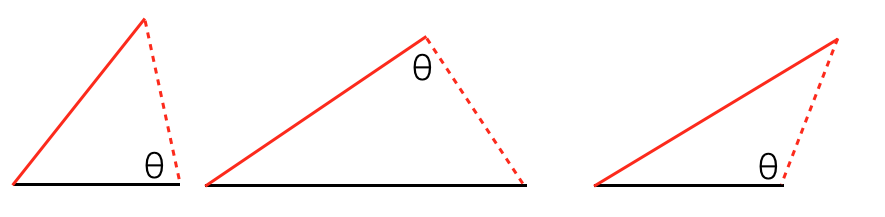
\includegraphics [scale=0.4] {tri_types.png} \end{center}

The acute triangle (left) has all three angles smaller than a right angle.  The right triangle, naturally, has one right angle.

We'll say a lot more about right triangles later.

Finally, an obtuse triangle has one angle larger than a right angle (right, above).

\subsection*{symmetry}

One can also talk about the situation where either two sides, or all three sides, have the same length.  

An equilateral triangle has all three sides the same, while an isosceles triangle has two sides the same length.

The most important consequence of three sides equal for an equilateral triangle, is rotational symmetry.  Three turns of $120$ degrees, and we're back where we started.

\begin{center} 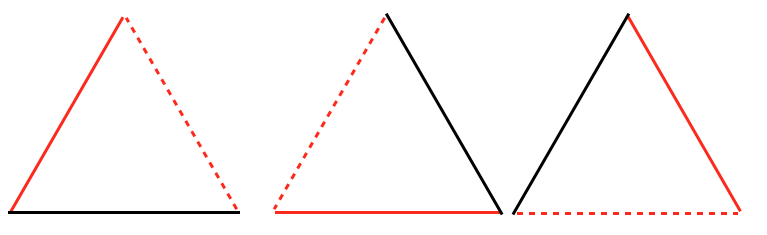
\includegraphics [scale=0.4] {equilateral.png} \end{center}

The implication of that is that the three angles are also equal.  There is no reason to choose one larger than any other.

A formal proof easily follows from the isosceles triangle theorem that we prove later in this chapter.

In the next figure the two smaller triangles obtained by dividing in half an equilateral triangle (all sides equal), are congruent.

\begin{center} 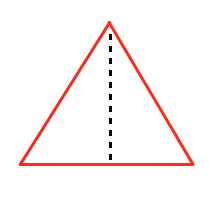
\includegraphics [scale=0.6] {congruent2.png} \end{center}

By divide in half, we mean bisect the base and draw the line from the top vertex.  We have SSS.

We also have that the two angles at the base of the bisector are equal and supplementary angles.  Therefore, they are both right angles.

$\square$

\subsection*{theorem from Thales}

$\bullet$  The base angles of an isosceles triangle are equal.  Also, if the two base angles are equal, the triangle is isosceles.

\begin{center} 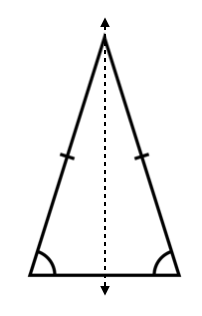
\includegraphics [scale=0.6] {isosceles.png} \end{center}

My favorite proof of this theorem is from reflective or mirror image symmetry (above).  

Start with the two sides equal and draw a line to the midpoint of the base opposite.  The figure has reflective symmetry, thus the angle is bisected.

We prove this more carefully now.

\subsection*{notation}

The Greeks, including Euclid, adhere to certain conventions.  For example, points are always labeled with letters, line segments are referred to by the endpoints, and angles by the line segments that determine them, as in $\angle ABC = \angle DEF$.

I don't know about you but I find myself tracing out angles from the three points, again and again.

We could give labels to the angles like $\alpha, \beta \dots$ and so on, to the sides opposite vertices as $a$ opposite $A$ and so on.  

Boldly, we choose to be even more dramatic.  Dispense with labels altogether and use colored dots for equal angles and colored bars for equal lengths.  

Here is the famous proof of Thales' theorem from Euclid's \emph{Elements}.

\subsection*{Euclid Prop. I.5}

In isosceles triangles the angles at the base equal one another, and, if the equal straight lines are produced further, then the angles under the base equal one another.

In what follows, all the pieces are with reference to the initial construction, first figure, below.

\begin{center} 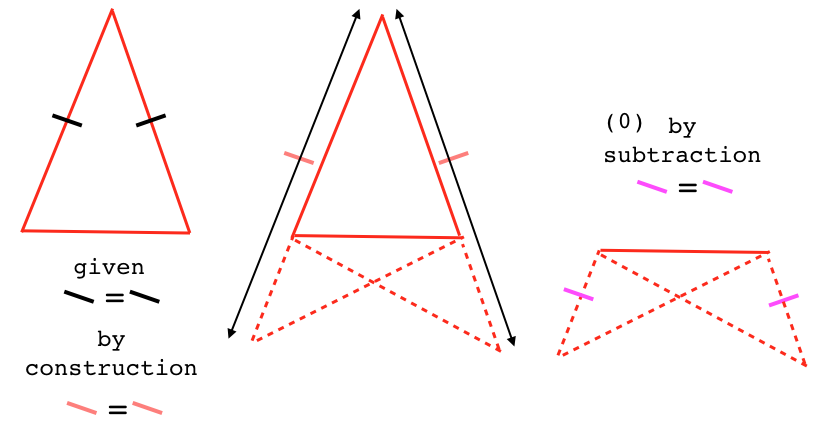
\includegraphics [scale=0.35] {PI_5d.png} \end{center}

\begin{center} 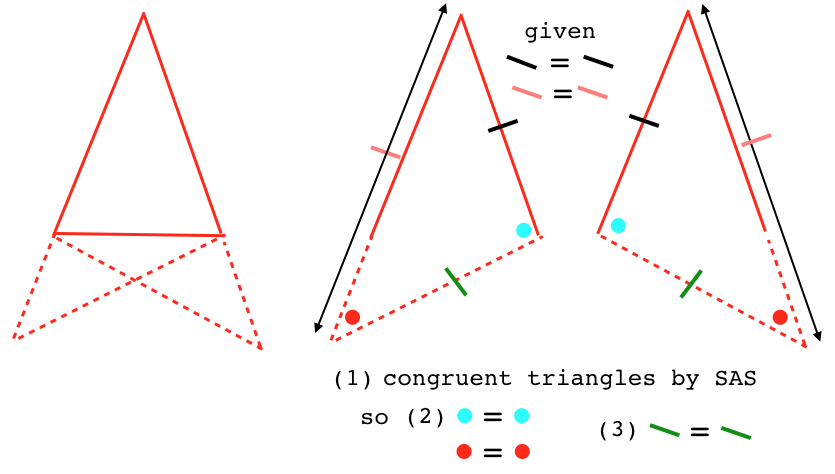
\includegraphics [scale=0.35] {PI_5e.png} \end{center}

\begin{center} 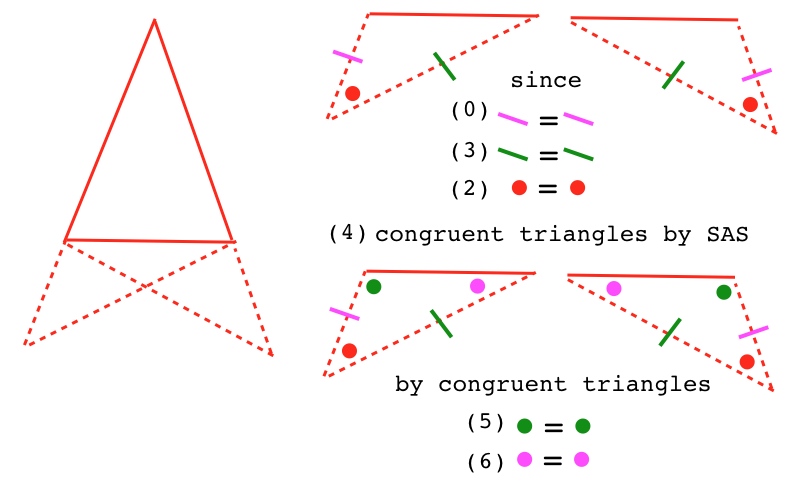
\includegraphics [scale=0.35] {PI_5f.png} \end{center}

\begin{center} 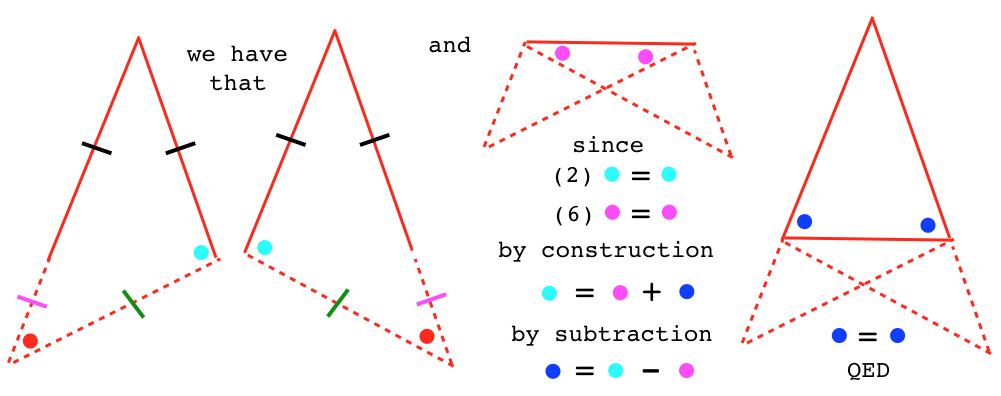
\includegraphics [scale=0.35] {PI_5g.png} \end{center}

$\square$

The theorem says that the base angles are equal $\iff$ the two sides sides are equal (not the base).  

The symbol $\iff$ means \emph{if and only if}, so $A \iff B$ means that both $A \rightarrow B$ and $B \rightarrow A$.

So far, our proof runs only in the forward direction.

In isosceles triangles the angles at the base equal one another, and, if the equal straight lines are produced further, then the angles under the base equal one another.

Euclid's proof of the converse is short and introduces the method of contradiction, or \emph{reductio ad absurdum}.  That is the next proposition.
  
\subsection*{Euclid Prop. I.6}

If in a triangle two angles equal one another, then the sides opposite the equal angles also equal one another.

Suppose we have $\triangle ABC$ with equal angles $\beta = \gamma$ at the base (left panel).

\begin{center} 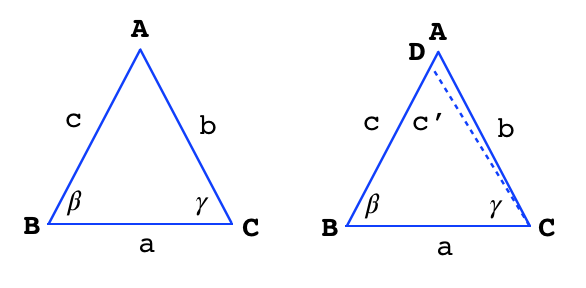
\includegraphics [scale=0.4] {PI_6b.png} \end{center}

We will assume that the two sides $b$ and $c$ are not equal.  Then one of them is greater.  Let $c$ be greater, then cut off $b$ from $c$ at point $D$ such that the new length $c' = b$.

The new triangle has sides $c'$ and $a$, which flank angle $\beta$, while for the original we have side $b$ and side $a$ flanking $\gamma$.   But we constructed $c' = b$, are given that $\beta = \gamma$, and the side $a$ is common.  

Therefore the $\triangle DBC \cong \triangle ACB$ by SAS.

But this means that the less equals the greater, which is absurd. 

Therefore $c$ cannot be unequal to $b$.  It therefore equals it.

Our original assumption that $b$ does not equal $c$ must be false.

$\square$

A corollary is that if a triangle has all three angles equal, then it is equilateral.

\subsection*{altitudes}

Above we said that in this figure the two smaller triangles obtained by dividing an equilateral triangle in half, are congruent.  The dotted line is called an \emph{altitude} of the triangle.

\begin{center} 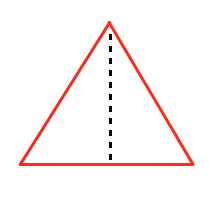
\includegraphics [scale=0.5] {congruent2.png} \end{center}

An altitude meets the side opposite in a right triangle.

Because the left and right sides of the original triangle are equal, the base angles are equal, by the property of isosceles triangles which we just proved.  The angles where the altitude meets the base are both right angles, by symmetry and by the definition of the altitude.  

Therefore we have AAS, and the two halves are congruent.

So, the two angles at the top where the altitude meets the sides are also equal (as the third angle with the other two angles determined).

\subsection*{note on proofs}

If you pick up a high school geometry textbook, you will see what they call \emph{two column} proofs, with the statement in one column and the reason in the second.  This is really just a matter of style.  

However, another thing you will see there that I don't care for is formal statements of things that are obvious, and these are required for \emph{every} proof.

Rather than say congruent triangles they will say:

$\circ$ \ CPCTC: corresponding parts of congruent triangles are congruent.

Or rather than say "side $a$ is shared" they say:

$\circ$ \ Reflexive property, and write $a = a$.

Or rather than say $AC = 2 AB$ so $AB = AC/2$ they wiqll say:

$\circ$ \ division property of the equals sign"

or some such.  If you have to say something, say "basic arithmetic."

This is completely unnecessary, unless of course you are taking such a course.



\end{document}